\documentclass[a4paper,12pt]{report}
\usepackage{graphicx}
\title{Resume Database Aplikasi Orecle}
\author{Nuha Hanifatul Khonsa'}
\date{ 1 November 2019}
\begin{document}


\maketitle

\section{Langkah dalam Pembuatan Aplikasi pada Orecle Apex}
\textit{Dalam membuat aplikasi menggunakan data mahasiswa dalam format excel pada orecle apex adalah sebagai beriku:}

\begin{enumerate}
    \item Hal pertama yang diperlukan ialah kita harus sudah memiliki akun orecle apex dan melakukan login dengan pilih sing in dan dilanjutkan dengan memasukkan workspace, username, dan password
    \begin{center}
    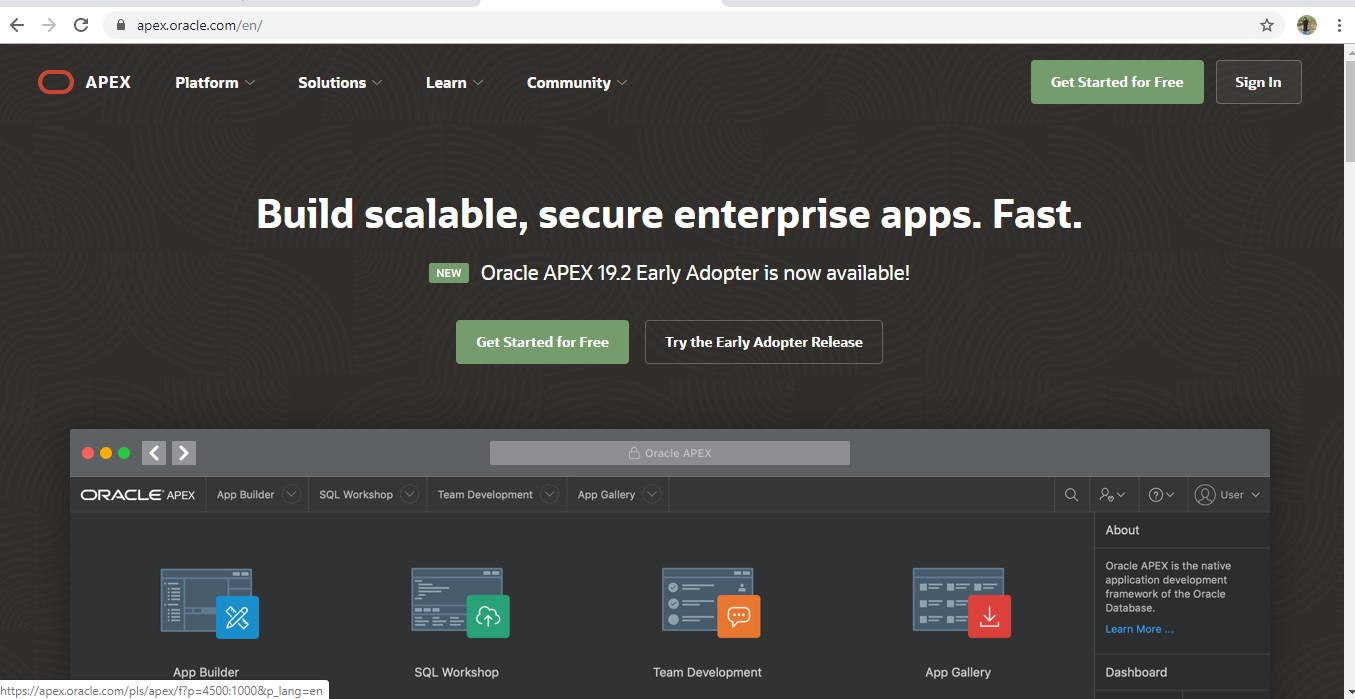
\includegraphics[width=11cm\textwidth]{figure/1.jpg}
    \end{center}
    \begin{center}
    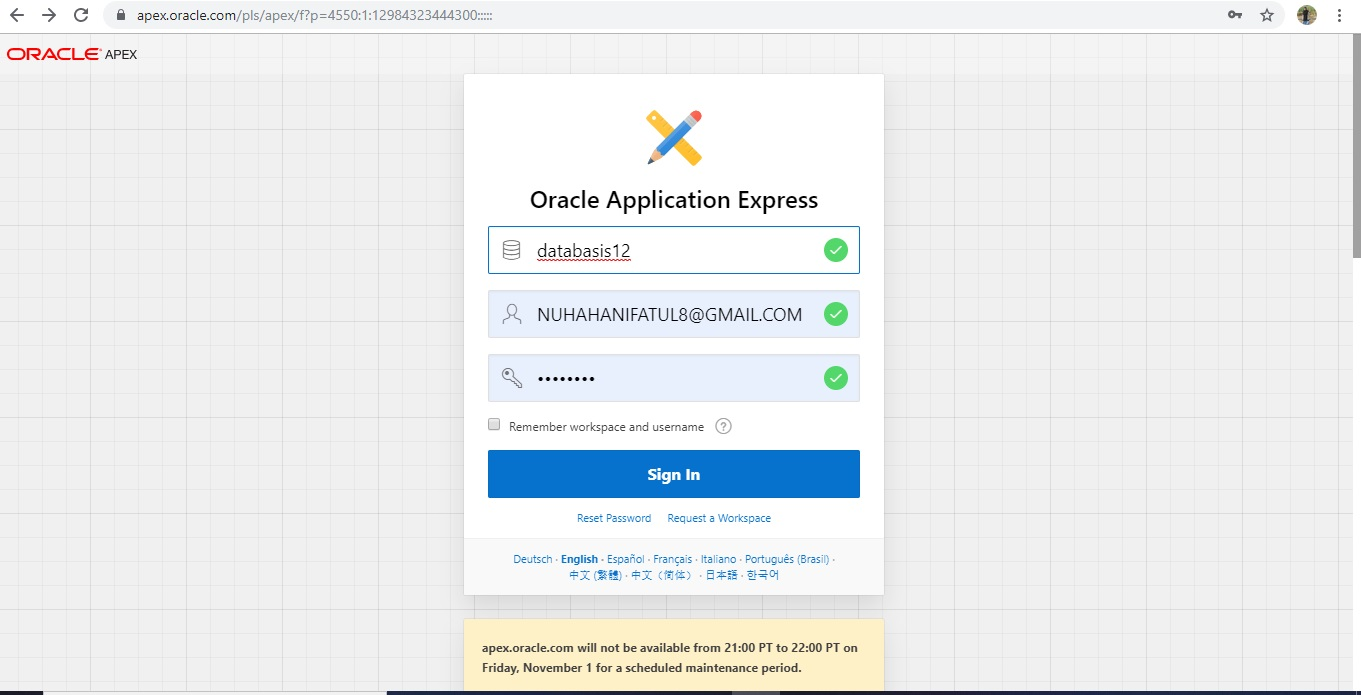
\includegraphics[width=11cm\textwidth]{figure/2.jpg}
    \end{center}
    \item Pilih App Builder untuk membuat aplikasi
    \begin{center}
    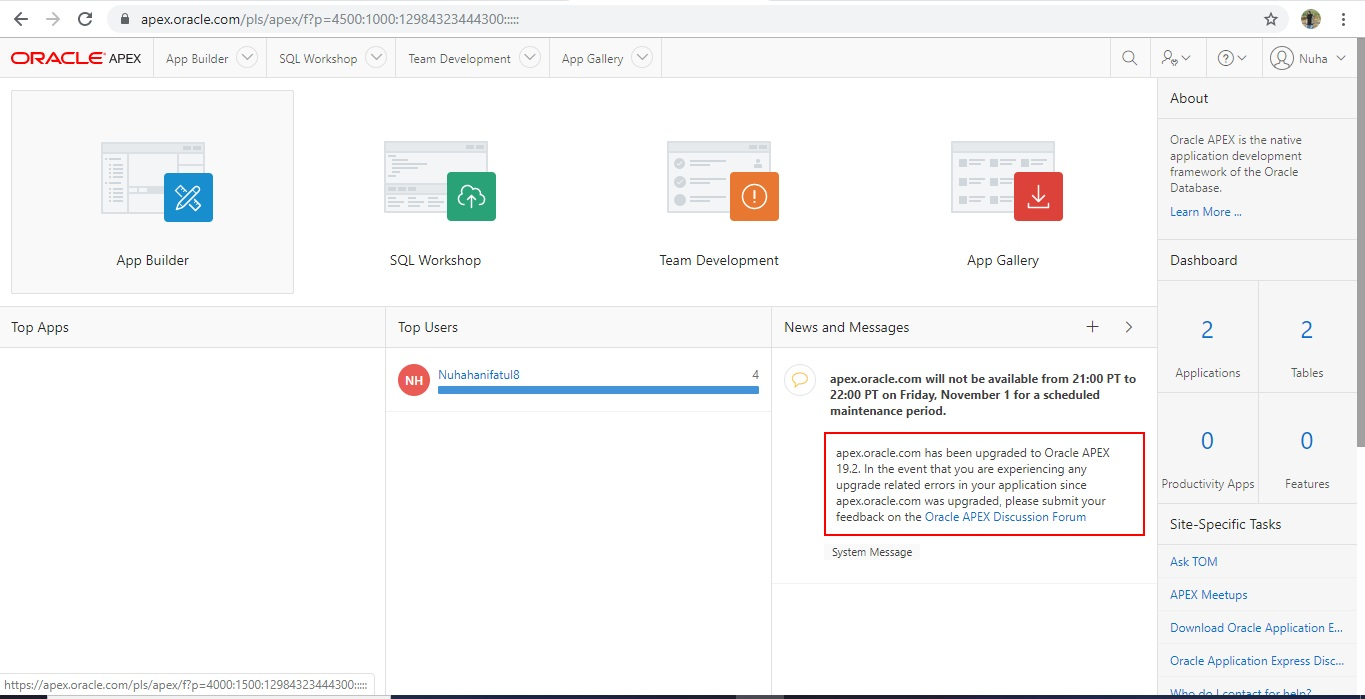
\includegraphics[width=11cm\textwidth]{figure/3.jpg}
    \end{center}
    \item Lalu pilih Create
    \begin{center}
    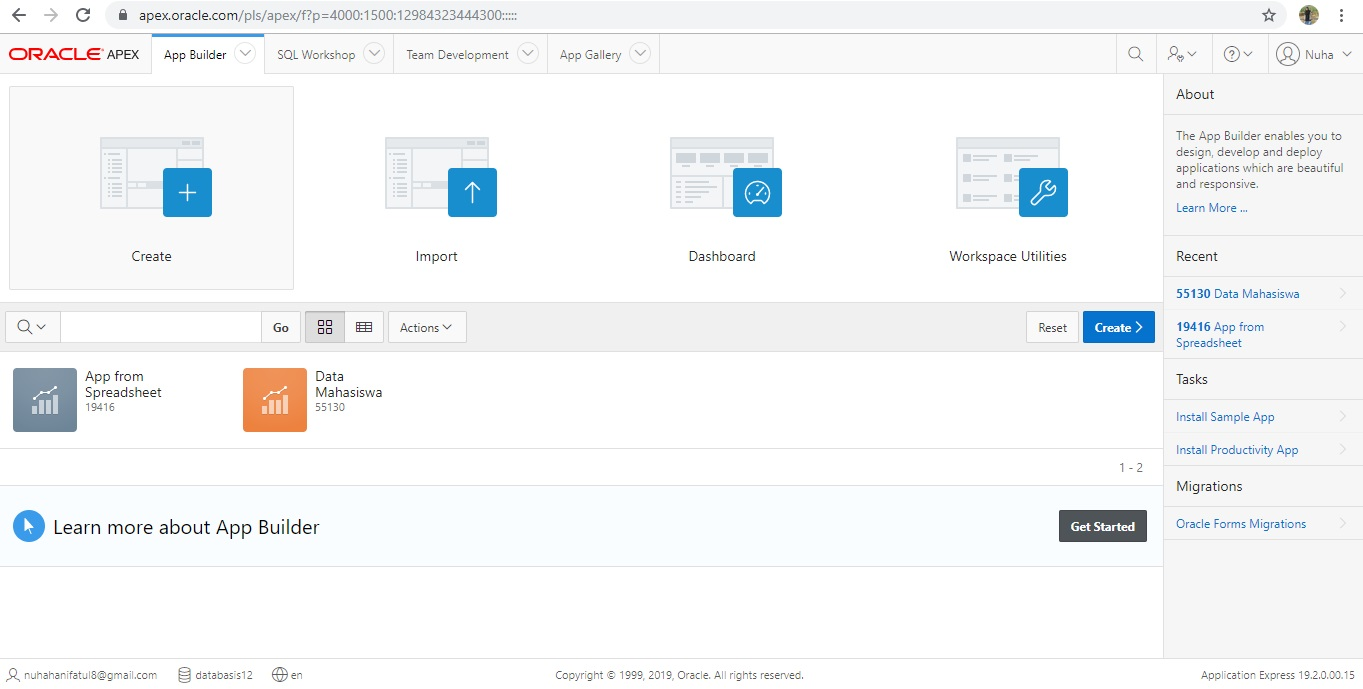
\includegraphics[width=11cm\textwidth]{figure/4.jpg}
    \end{center}
    \item Kemudian Pilih From a File
    \begin{center}
    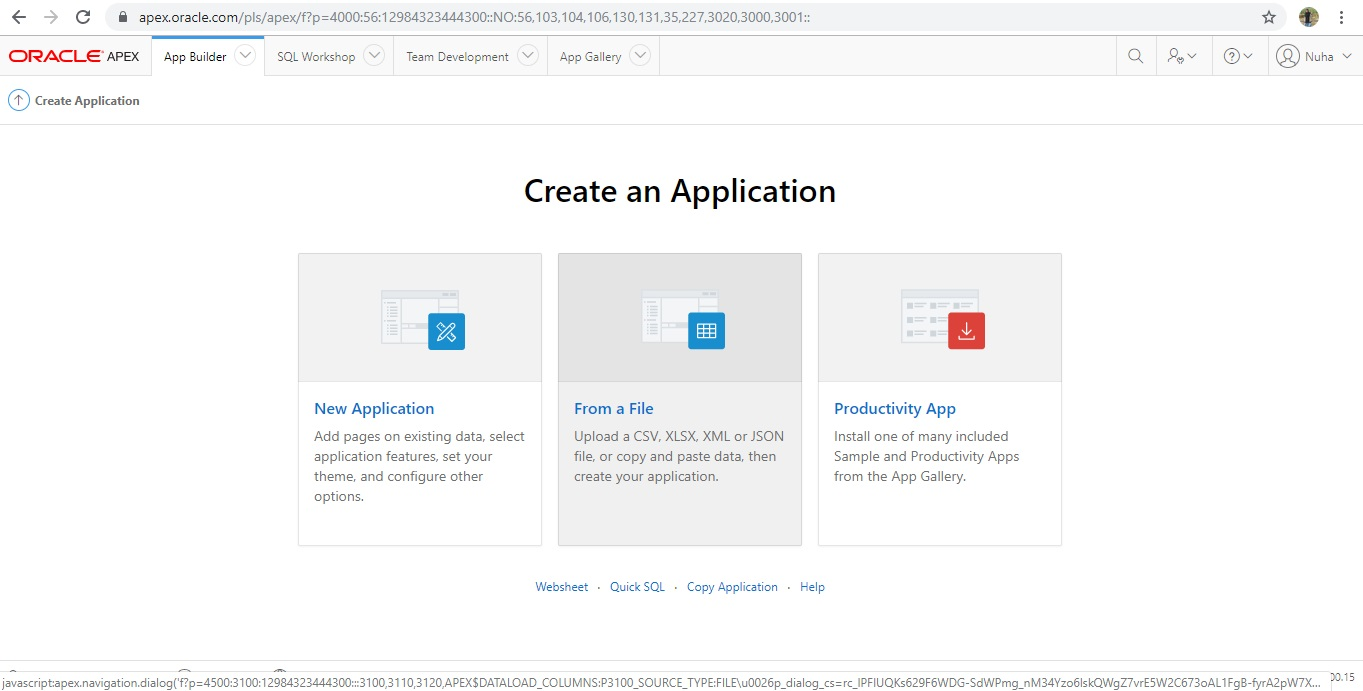
\includegraphics[width=11cm\textwidth]{figure/5.jpg}
    \end{center}
    \item Upload File lalu Chose a File pilih data file yang mau di masukkan seperti data mahasiswa lalu load Data
    \begin{center}
    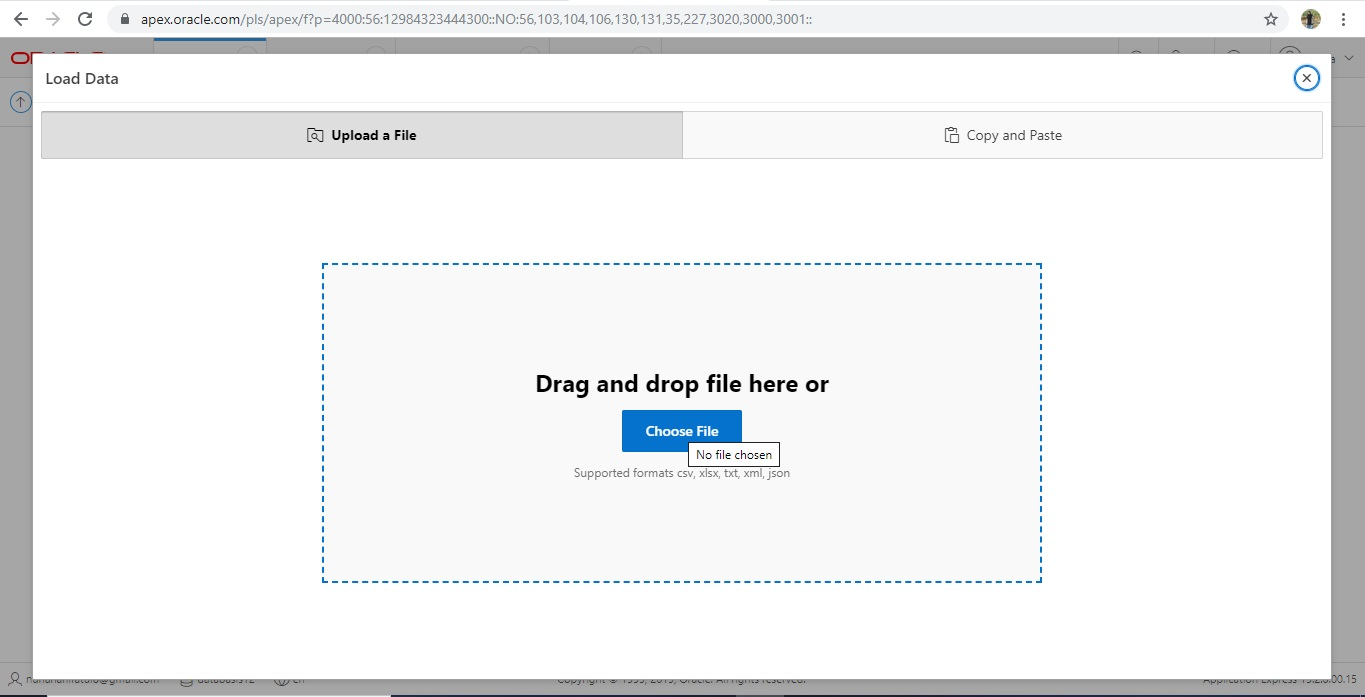
\includegraphics[width=11cm\textwidth]{figure/6.jpg}
    \end{center}
    \item cek data 50 rows seperti data yang ada lalu create aplication
    \begin{center}
    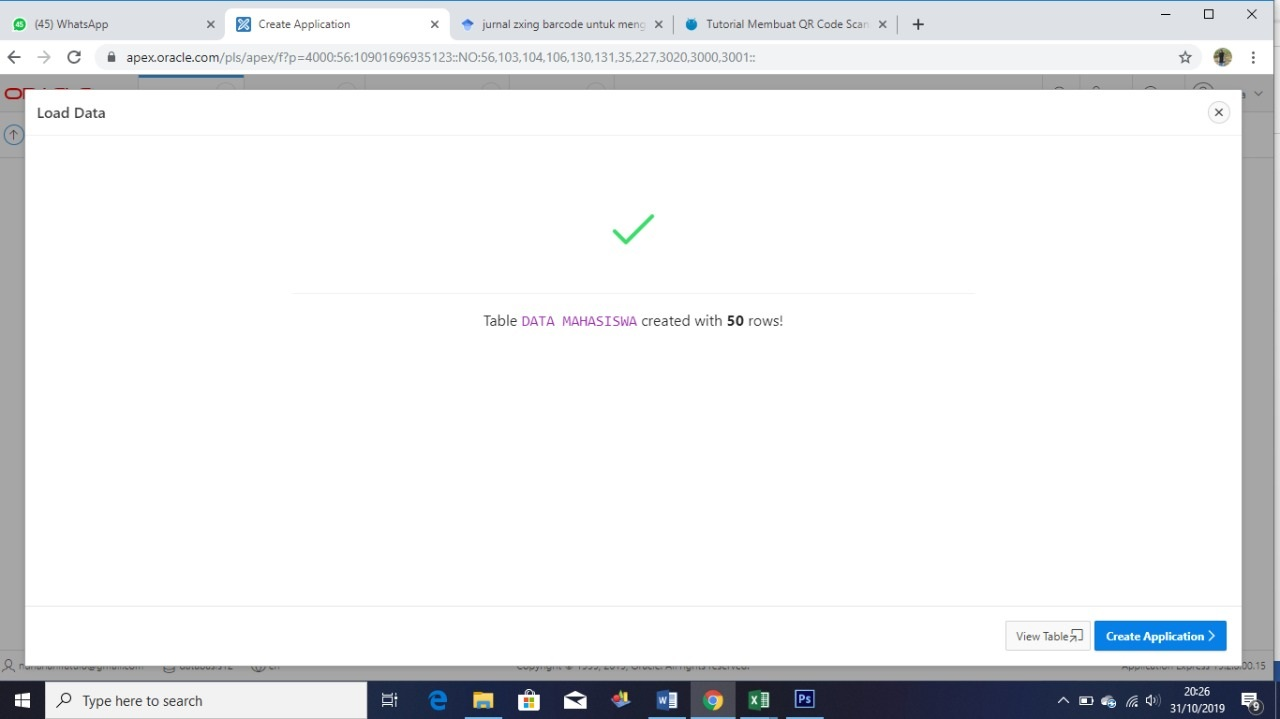
\includegraphics[width=11cm\textwidth]{figure/6.1.jpg}
    \end{center}
    \item Lalu beri nama tabel
    \begin{center}
    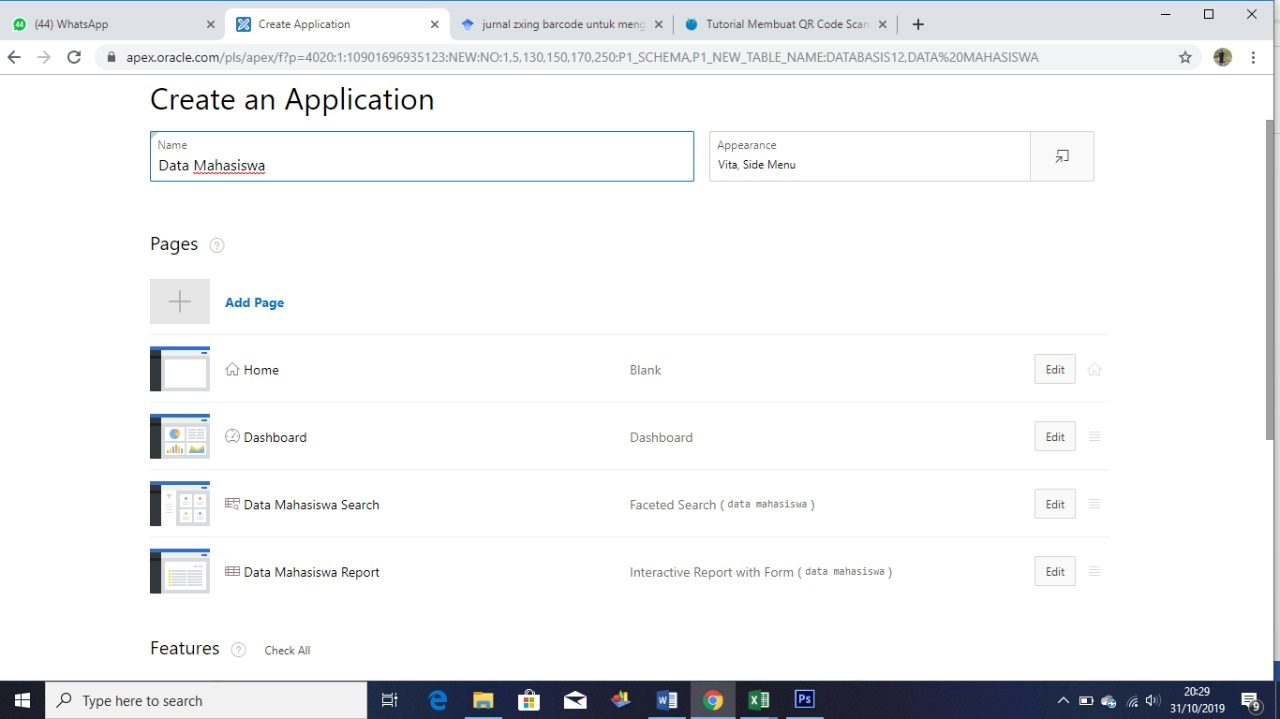
\includegraphics[width=11cm\textwidth]{figure/7.jpg}
    \end{center}
    \item Jangan lupa untuk pilih Check all Features lalu load data
    \begin{center}
    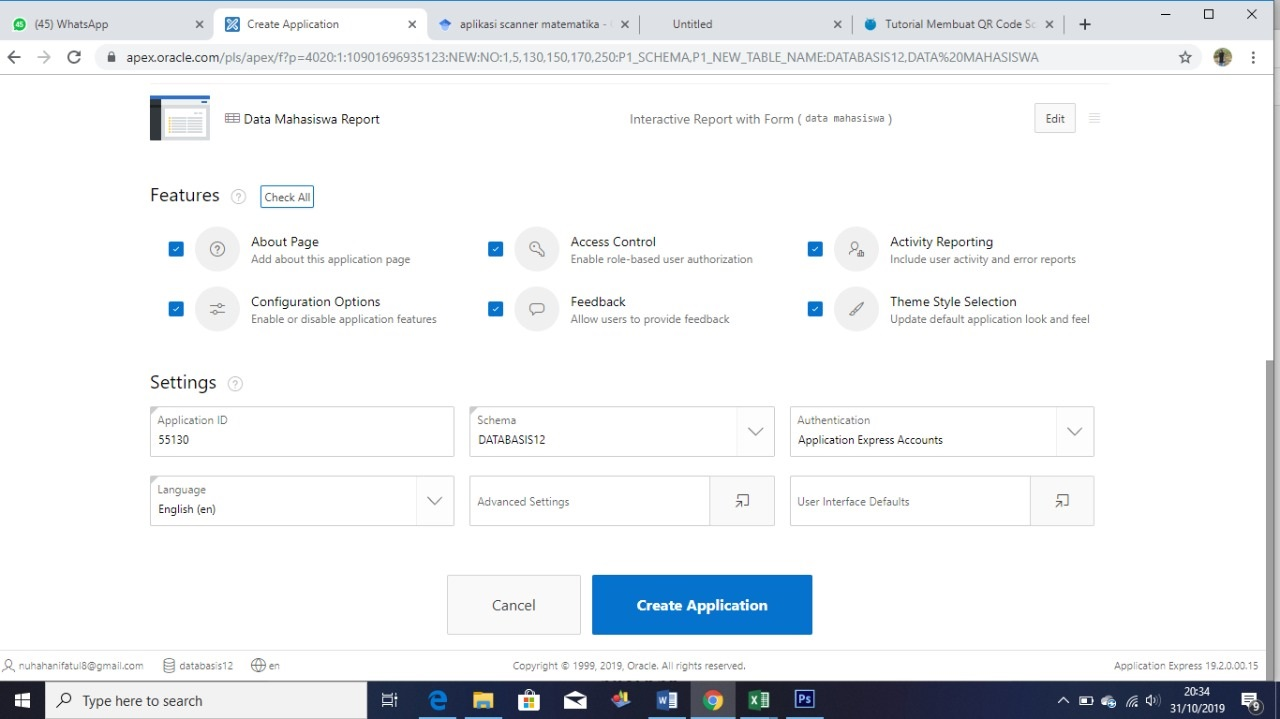
\includegraphics[width=11cm\textwidth]{figure/8.jpg}
    \end{center}
    \begin{center}
    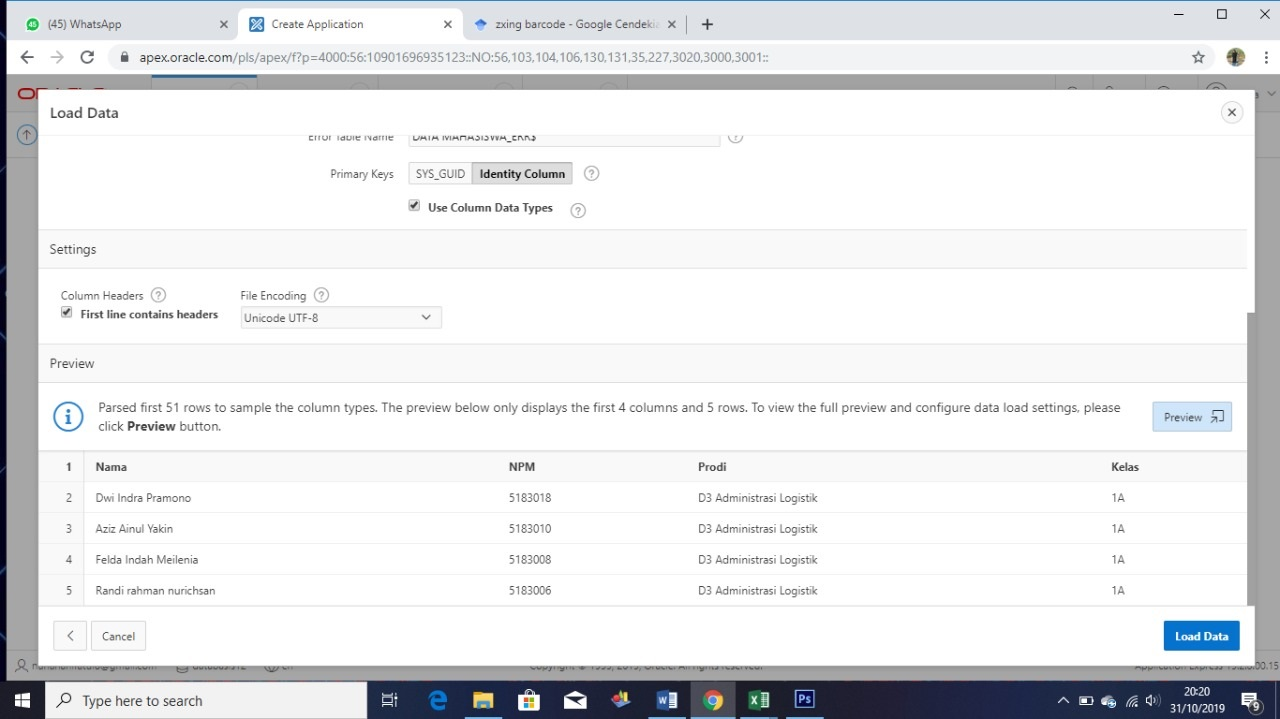
\includegraphics[width=11cm\textwidth]{figure/9.jpg}
    \end{center}
    \item Lalu untuk menjalankan aplikasi pilih Run aplikasi
    \begin{center}
    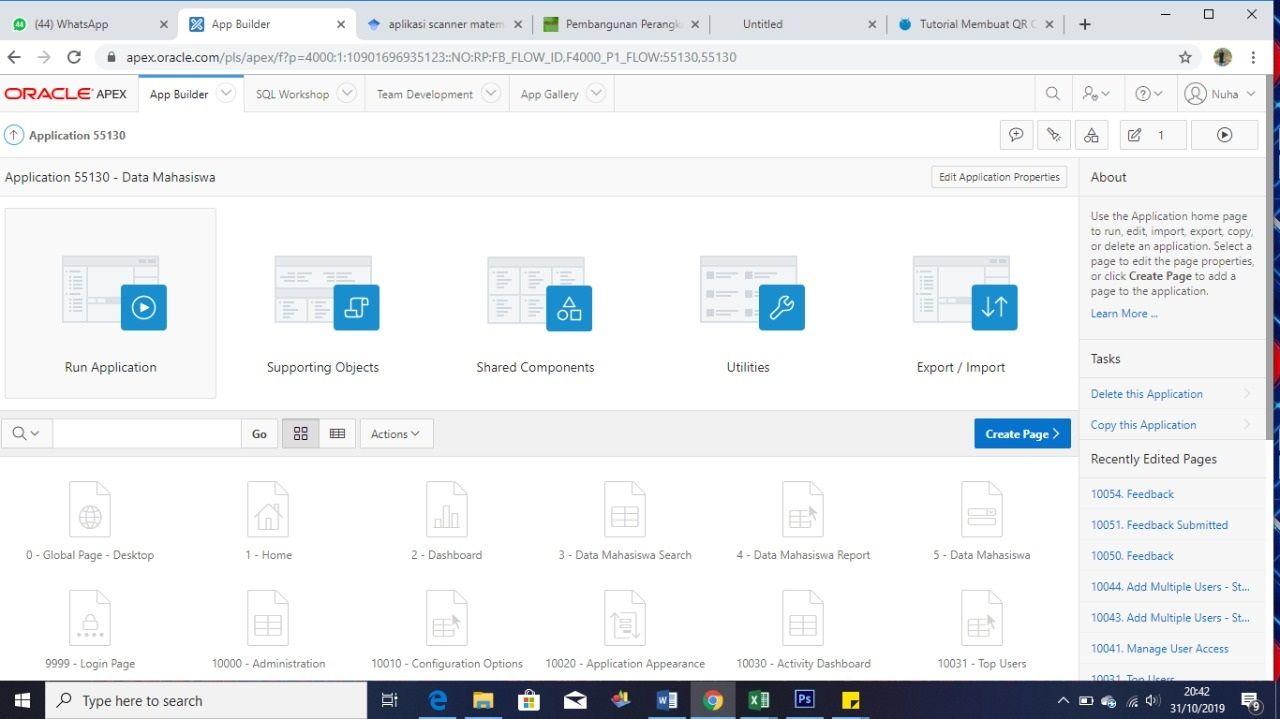
\includegraphics[width=11cm\textwidth]{figure/10.jpg}
    \end{center}
    \item masukkan user credensial anda
    \begin{center}
    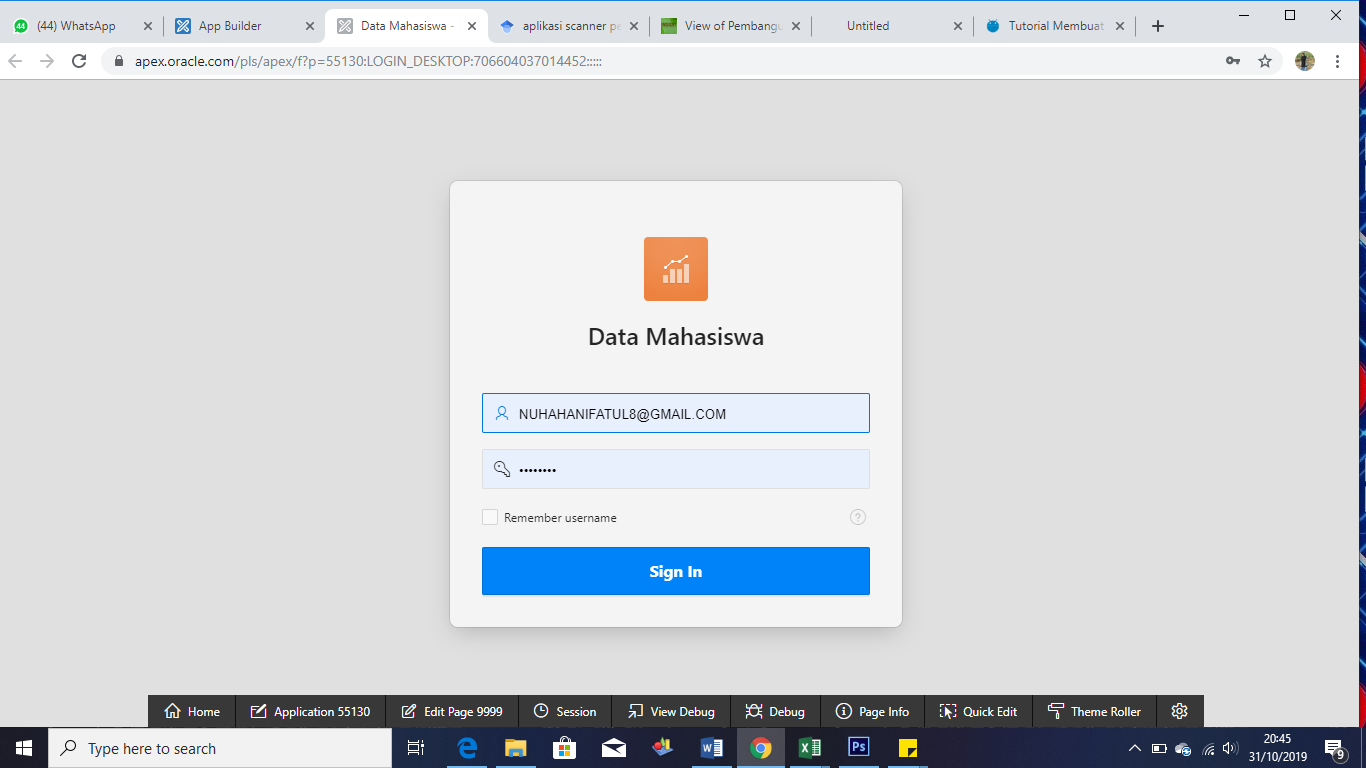
\includegraphics[width=11cm\textwidth]{figure/user.png}
    \end{center}
    \item Aplikasi anda sudah jadi
    \begin{center}
    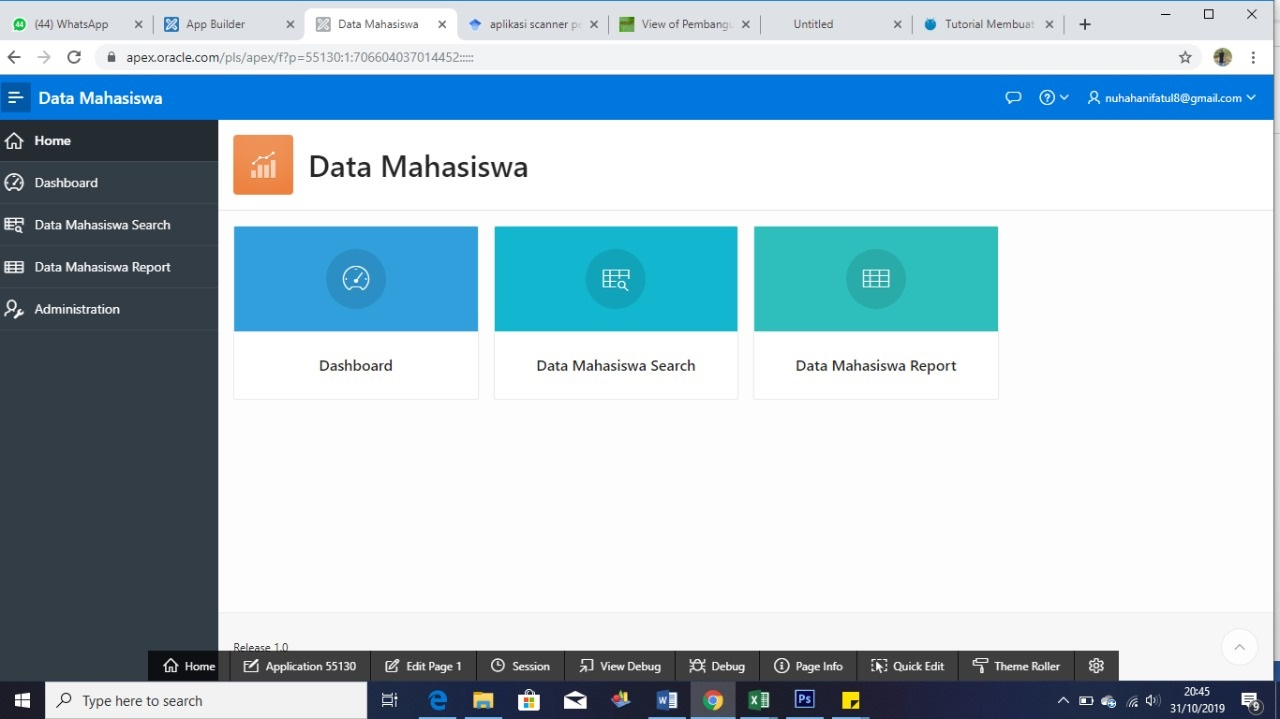
\includegraphics[width=11cm\textwidth]{figure/11.jpg}
    \end{center}
\end{enumerate}


    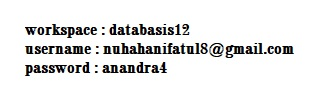
\includegraphics[width=6cm\textwidth]{figure/nuha.jpg}


\end{document}
